% \section{IMU误差模型}

\begin{comment}
\end{comment}
\begin{frame}
\frametitle{确定性误差标定 \hfill 
\includegraphics[height=0.5cm]{00_logo.png}}
\begin{columns}
  \column{0.1\textwidth}
  
  \column{0.8\textwidth}
  六面法标定加速度计Bias/Scale和Nonorthogonality.

  六面法:将加速度计的3个轴分别朝上或朝下水平放置一段时间,采集6个面的数据完成标定.
	\begin{enumerate}
		\item 如果各个轴是正交的,那么很容易得到bias和scale:
		\begin{equation}
      \begin{split}
          &b = \frac{l^{up}_f + l^{down}_f}{2} \\
          & S = \frac{l^{up}_f - l^{down}_f}{2 \cdot ||g||}
      \end{split}
    \end{equation}

    其中,l为加速度计某个轴的测量值,g为当地的重力加速度.

  \end{enumerate}
  
  % \column{0.3\textwidth}
	% \begin{figure}[h]
	% 	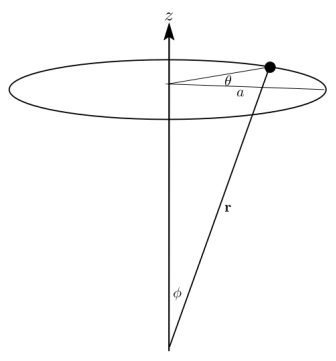
\includegraphics[trim=1.5 0 0 0, height=3.5cm,clip]{11_0.png}
	% 	% \caption{四个区域搜索空间}
  % \end{figure}
  
	\column{0.1\textwidth}

\end{columns}
\end{frame}

%%%%%%%%%%%%%%%%%%%%%%%%%%%%

\begin{comment}
\end{comment}
\begin{frame}
\frametitle{确定性误差标定 \hfill 
\includegraphics[height=0.5cm]{00_logo.png}}
\begin{columns}
  \column{0.1\textwidth}
  
  \column{0.8\textwidth}
  
  \begin{enumerate}
    \setcounter{enumi}{1}
		\item 考虑轴间误差的时候,实际加速度和测量值之间的关系为:
		\begin{equation}
      \begin{split}
        \begin{bmatrix}
          l_{ax} \\ l_{ay} \\ l_{az}
        \end{bmatrix} = 
        \begin{bmatrix}
          b_{ax} \\ b_{ay} \\ b_{az}
        \end{bmatrix} +
        \begin{bmatrix}
          s_{xx} & m_{xy} & m_{xz} \\
          m_{yx} & s_{yy} & m_{yz} \\
          m_{zx} & m_{zy} & s_{zz}
        \end{bmatrix} \cdot 
        \begin{bmatrix}
          a_x \\ a_y \\ a_z
        \end{bmatrix}
      \end{split}
    \end{equation}

    水平静止放置6面的时候,加速度的理论值为:

    \begin{equation}
      a1 = \begin{bmatrix}
        g \\ 0 \\ 0
      \end{bmatrix},
      a2 = \begin{bmatrix}
        -g \\ 0 \\ 0
      \end{bmatrix},
      a3 = \begin{bmatrix}
        0 \\ g \\ 0
      \end{bmatrix},
      a4 = \begin{bmatrix}
        0 \\ -g \\ 0
      \end{bmatrix},
      a5 = \begin{bmatrix}
        0 \\ 0 \\ g
      \end{bmatrix},
      a6 = \begin{bmatrix}
        0 \\ 0 \\ -g
      \end{bmatrix}
    \end{equation}

    其中,l为加速度计某个轴的测量值,g为当地的重力加速度.

    对应的测量值矩阵L:
    \begin{equation}
      L = [I_1, I_2,I_3,I_4,I_5, I_6]  
    \end{equation}

    利用最小二乘就能够把12个变量求出来.

  \end{enumerate}
  
  % \column{0.3\textwidth}
	% \begin{figure}[h]
	% 	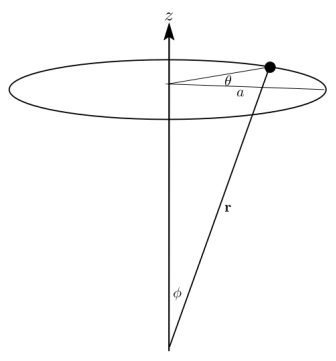
\includegraphics[trim=1.5 0 0 0, height=3.5cm,clip]{11_0.png}
	% 	% \caption{四个区域搜索空间}
  % \end{figure}
  
	\column{0.1\textwidth}

\end{columns}
\end{frame} 



%%%%%%%%%%%%%%%%%%%%%%%%%%%%

\begin{comment}
\end{comment}
\begin{frame}
\frametitle{确定性误差标定 \hfill 
\includegraphics[height=0.5cm]{00_logo.png}}
\begin{columns}
  \column{0.1\textwidth}
  
  \column{0.5\textwidth}
  六面法标定陀螺Bias/Scale和Nonorthogonality.
  
  \begin{itemize}
    \item 和加速度计六面法不同的是,陀螺仪的真实值由高精度转台提供,这里的6面是指各个轴顺时针和逆时针旋转.
  \end{itemize}
  
  \column{0.3\textwidth}
	\begin{figure}[h]
		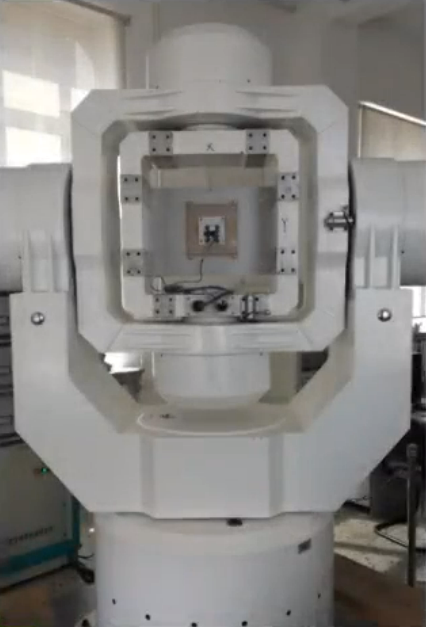
\includegraphics[trim=1.5 0 0 0, height=3.5cm,clip]{12_1.png}
		% \caption{四个区域搜索空间}
  \end{figure}
  
	\column{0.1\textwidth}

\end{columns}
\end{frame} 
